\documentclass[1p]{elsarticle_modified}
%\bibliographystyle{elsarticle-num}

%\usepackage[colorlinks]{hyperref}
%\usepackage{abbrmath_seonhwa} %\Abb, \Ascr, \Acal ,\Abf, \Afrak
\usepackage{amsfonts}
\usepackage{amssymb}
\usepackage{amsmath}
\usepackage{amsthm}
\usepackage{scalefnt}
\usepackage{amsbsy}
\usepackage{kotex}
\usepackage{caption}
\usepackage{subfig}
\usepackage{color}
\usepackage{graphicx}
\usepackage{xcolor} %% white, black, red, green, blue, cyan, magenta, yellow
\usepackage{float}
\usepackage{setspace}
\usepackage{hyperref}

\usepackage{tikz}
\usetikzlibrary{arrows}

\usepackage{multirow}
\usepackage{array} % fixed length table
\usepackage{hhline}

%%%%%%%%%%%%%%%%%%%%%
\makeatletter
\renewcommand*\env@matrix[1][\arraystretch]{%
	\edef\arraystretch{#1}%
	\hskip -\arraycolsep
	\let\@ifnextchar\new@ifnextchar
	\array{*\c@MaxMatrixCols c}}
\makeatother %https://tex.stackexchange.com/questions/14071/how-can-i-increase-the-line-spacing-in-a-matrix
%%%%%%%%%%%%%%%

\usepackage[normalem]{ulem}

\newcommand{\msout}[1]{\ifmmode\text{\sout{\ensuremath{#1}}}\else\sout{#1}\fi}
%SOURCE: \msout is \stkout macro in https://tex.stackexchange.com/questions/20609/strikeout-in-math-mode

\newcommand{\cancel}[1]{
	\ifmmode
	{\color{red}\msout{#1}}
	\else
	{\color{red}\sout{#1}}
	\fi
}

\newcommand{\add}[1]{
	{\color{blue}\uwave{#1}}
}

\newcommand{\replace}[2]{
	\ifmmode
	{\color{red}\msout{#1}}{\color{blue}\uwave{#2}}
	\else
	{\color{red}\sout{#1}}{\color{blue}\uwave{#2}}
	\fi
}

\newcommand{\Sol}{\mathcal{S}} %segment
\newcommand{\D}{D} %diagram
\newcommand{\A}{\mathcal{A}} %arc


%%%%%%%%%%%%%%%%%%%%%%%%%%%%%5 test

\def\sl{\operatorname{\textup{SL}}(2,\Cbb)}
\def\psl{\operatorname{\textup{PSL}}(2,\Cbb)}
\def\quan{\mkern 1mu \triangleright \mkern 1mu}

\theoremstyle{definition}
\newtheorem{thm}{Theorem}[section]
\newtheorem{prop}[thm]{Proposition}
\newtheorem{lem}[thm]{Lemma}
\newtheorem{ques}[thm]{Question}
\newtheorem{cor}[thm]{Corollary}
\newtheorem{defn}[thm]{Definition}
\newtheorem{exam}[thm]{Example}
\newtheorem{rmk}[thm]{Remark}
\newtheorem{alg}[thm]{Algorithm}

\newcommand{\I}{\sqrt{-1}}
\begin{document}

%\begin{frontmatter}
%
%\title{Boundary parabolic representations of knots up to 8 crossings}
%
%%% Group authors per affiliation:
%\author{Yunhi Cho} 
%\address{Department of Mathematics, University of Seoul, Seoul, Korea}
%\ead{yhcho@uos.ac.kr}
%
%
%\author{Seonhwa Kim} %\fnref{s_kim}}
%\address{Center for Geometry and Physics, Institute for Basic Science, Pohang, 37673, Korea}
%\ead{ryeona17@ibs.re.kr}
%
%\author{Hyuk Kim}
%\address{Department of Mathematical Sciences, Seoul National University, Seoul 08826, Korea}
%\ead{hyukkim@snu.ac.kr}
%
%\author{Seokbeom Yoon}
%\address{Department of Mathematical Sciences, Seoul National University, Seoul, 08826,  Korea}
%\ead{sbyoon15@snu.ac.kr}
%
%\begin{abstract}
%We find all boundary parabolic representation of knots up to 8 crossings.
%
%\end{abstract}
%\begin{keyword}
%    \MSC[2010] 57M25 
%\end{keyword}
%
%\end{frontmatter}

%\linenumbers
%\tableofcontents
%
\newcommand\colored[1]{\textcolor{white}{\rule[-0.35ex]{0.8em}{1.4ex}}\kern-0.8em\color{red} #1}%
%\newcommand\colored[1]{\textcolor{white}{ #1}\kern-2.17ex	\textcolor{white}{ #1}\kern-1.81ex	\textcolor{white}{ #1}\kern-2.15ex\color{red}#1	}

{\Large $\underline{12a_{1074}~(K12a_{1074})}$}

\setlength{\tabcolsep}{10pt}
\renewcommand{\arraystretch}{1.6}
\vspace{1cm}\begin{tabular}{m{100pt}>{\centering\arraybackslash}m{274pt}}
\multirow{5}{120pt}{
	\centering
	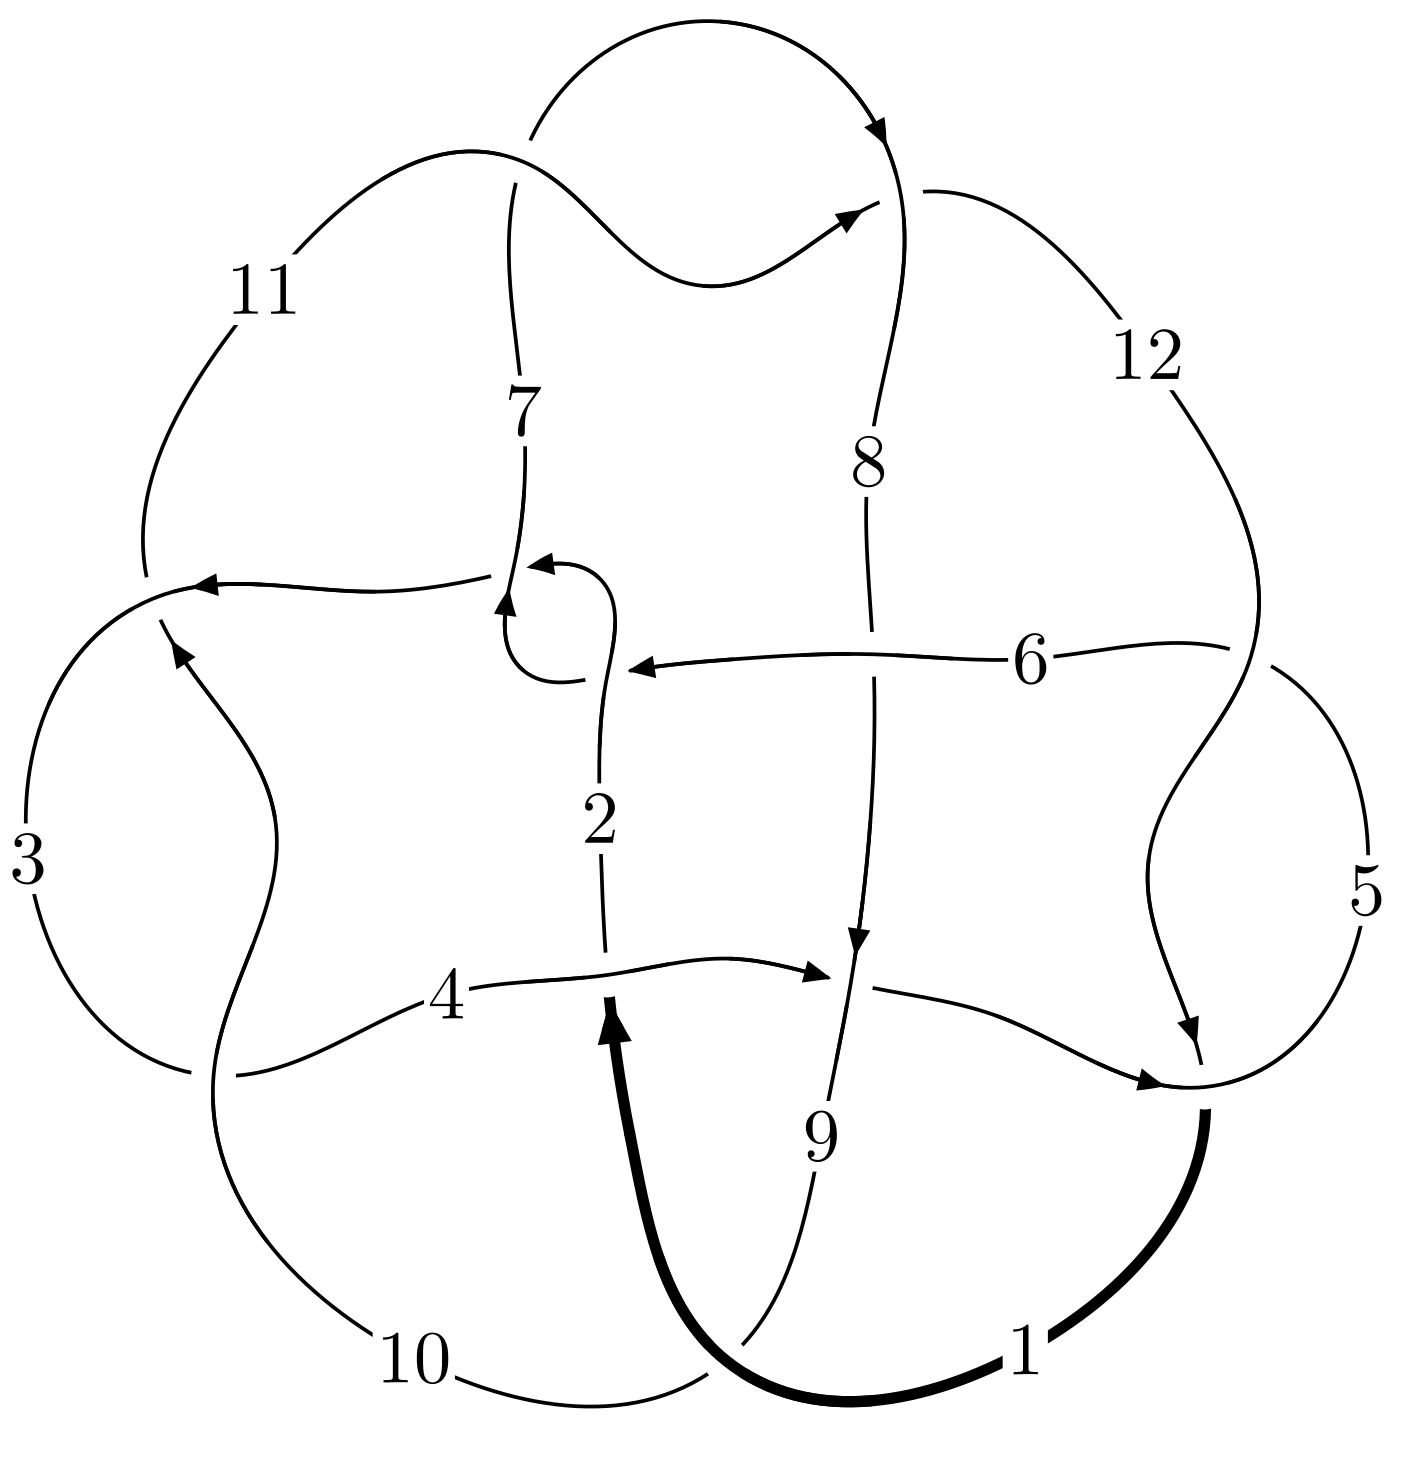
\includegraphics[width=112pt]{../../../GIT/diagram.site/Diagrams/png/1875_12a_1074.png}\\
\ \ \ A knot diagram\footnotemark}&
\allowdisplaybreaks
\textbf{Linearized knot diagam} \\
\cline{2-2}
 &
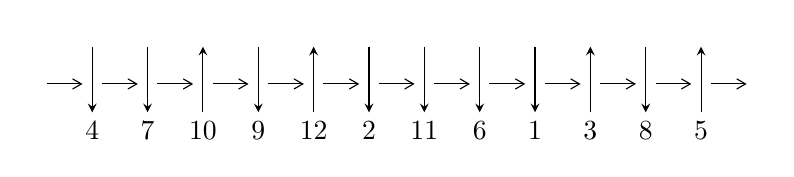
\begin{tikzpicture}[x=20pt, y=17pt]
	% nodes
	\node (C0) at (0, 0) {};
	\node (C1) at (1, 0) {};
	\node (C1U) at (1, +1) {};
	\node (C1D) at (1, -1) {4};

	\node (C2) at (2, 0) {};
	\node (C2U) at (2, +1) {};
	\node (C2D) at (2, -1) {7};

	\node (C3) at (3, 0) {};
	\node (C3U) at (3, +1) {};
	\node (C3D) at (3, -1) {10};

	\node (C4) at (4, 0) {};
	\node (C4U) at (4, +1) {};
	\node (C4D) at (4, -1) {9};

	\node (C5) at (5, 0) {};
	\node (C5U) at (5, +1) {};
	\node (C5D) at (5, -1) {12};

	\node (C6) at (6, 0) {};
	\node (C6U) at (6, +1) {};
	\node (C6D) at (6, -1) {2};

	\node (C7) at (7, 0) {};
	\node (C7U) at (7, +1) {};
	\node (C7D) at (7, -1) {11};

	\node (C8) at (8, 0) {};
	\node (C8U) at (8, +1) {};
	\node (C8D) at (8, -1) {6};

	\node (C9) at (9, 0) {};
	\node (C9U) at (9, +1) {};
	\node (C9D) at (9, -1) {1};

	\node (C10) at (10, 0) {};
	\node (C10U) at (10, +1) {};
	\node (C10D) at (10, -1) {3};

	\node (C11) at (11, 0) {};
	\node (C11U) at (11, +1) {};
	\node (C11D) at (11, -1) {8};

	\node (C12) at (12, 0) {};
	\node (C12U) at (12, +1) {};
	\node (C12D) at (12, -1) {5};
	\node (C13) at (13, 0) {};

	% arrows
	\draw[->,>={angle 60}]
	(C0) edge (C1) (C1) edge (C2) (C2) edge (C3) (C3) edge (C4) (C4) edge (C5) (C5) edge (C6) (C6) edge (C7) (C7) edge (C8) (C8) edge (C9) (C9) edge (C10) (C10) edge (C11) (C11) edge (C12) (C12) edge (C13) ;	\draw[->,>=stealth]
	(C1U) edge (C1D) (C2U) edge (C2D) (C3D) edge (C3U) (C4U) edge (C4D) (C5D) edge (C5U) (C6U) edge (C6D) (C7U) edge (C7D) (C8U) edge (C8D) (C9U) edge (C9D) (C10D) edge (C10U) (C11U) edge (C11D) (C12D) edge (C12U) ;
	\end{tikzpicture} \\
\hhline{~~} \\& 
\textbf{Solving Sequence} \\ \cline{2-2} 
 &
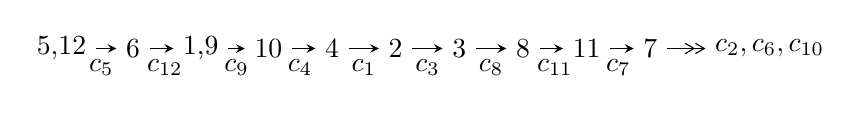
\begin{tikzpicture}[x=23pt, y=7pt]
	% node
	\node (A0) at (-1/8, 0) {5,12};
	\node (A1) at (1, 0) {6};
	\node (A2) at (33/16, 0) {1,9};
	\node (A3) at (25/8, 0) {10};
	\node (A4) at (33/8, 0) {4};
	\node (A5) at (41/8, 0) {2};
	\node (A6) at (49/8, 0) {3};
	\node (A7) at (57/8, 0) {8};
	\node (A8) at (65/8, 0) {11};
	\node (A9) at (73/8, 0) {7};
	\node (C1) at (1/2, -1) {$c_{5}$};
	\node (C2) at (3/2, -1) {$c_{12}$};
	\node (C3) at (21/8, -1) {$c_{9}$};
	\node (C4) at (29/8, -1) {$c_{4}$};
	\node (C5) at (37/8, -1) {$c_{1}$};
	\node (C6) at (45/8, -1) {$c_{3}$};
	\node (C7) at (53/8, -1) {$c_{8}$};
	\node (C8) at (61/8, -1) {$c_{11}$};
	\node (C9) at (69/8, -1) {$c_{7}$};
	\node (A10) at (11, 0) {$c_{2},c_{6},c_{10}$};

	% edge
	\draw[->,>=stealth]	
	(A0) edge (A1) (A1) edge (A2) (A2) edge (A3) (A3) edge (A4) (A4) edge (A5) (A5) edge (A6) (A6) edge (A7) (A7) edge (A8) (A8) edge (A9) ;
	\draw[->>,>={angle 60}]	
	(A9) edge (A10);
\end{tikzpicture} \\ 

\end{tabular} \\

\footnotetext{
The image of knot diagram is generated by the software ``\textbf{Draw programme}" developed by Andrew Bartholomew(\url{http://www.layer8.co.uk/maths/draw/index.htm\#Running-draw}), where we modified some parts for our purpose(\url{https://github.com/CATsTAILs/LinksPainter}).
}\phantom \\ \newline 
\centering \textbf{Ideals for irreducible components\footnotemark of $X_{\text{par}}$} 
 
\begin{align*}
I^u_{1}&=\langle 
-2.13559\times10^{526} u^{120}-5.74073\times10^{526} u^{119}+\cdots+1.31201\times10^{528} b-3.70864\times10^{528},\\
\phantom{I^u_{1}}&\phantom{= \langle  }-2.82909\times10^{528} u^{120}-9.33657\times10^{528} u^{119}+\cdots+2.37473\times10^{530} a-1.67417\times10^{531},\\
\phantom{I^u_{1}}&\phantom{= \langle  }u^{121}+3 u^{120}+\cdots+1450 u-181\rangle \\
I^u_{2}&=\langle 
-2231694469 u^{20}-1226056090 u^{19}+\cdots+4164425005 b-7694689318,\\
\phantom{I^u_{2}}&\phantom{= \langle  }-4558154114 u^{20}-8410552925 u^{19}+\cdots+4164425005 a-26590478038,\\
\phantom{I^u_{2}}&\phantom{= \langle  }u^{21}+2 u^{20}+\cdots+10 u-1\rangle \\
I^u_{3}&=\langle 
a u+b+u-1,\;3 a^2+5 a u- a- u-1,\;u^2- u+1\rangle \\
\\
\end{align*}
\raggedright * 3 irreducible components of $\dim_{\mathbb{C}}=0$, with total 146 representations.\\
\footnotetext{All coefficients of polynomials are rational numbers. But the coefficients are sometimes approximated in decimal forms when there is not enough margin.}
\newpage
\renewcommand{\arraystretch}{1}
\centering \section*{I. $I^u_{1}= \langle -2.14\times10^{526} u^{120}-5.74\times10^{526} u^{119}+\cdots+1.31\times10^{528} b-3.71\times10^{528},\;-2.83\times10^{528} u^{120}-9.34\times10^{528} u^{119}+\cdots+2.37\times10^{530} a-1.67\times10^{531},\;u^{121}+3 u^{120}+\cdots+1450 u-181 \rangle$}
\flushleft \textbf{(i) Arc colorings}\\
\begin{tabular}{m{7pt} m{180pt} m{7pt} m{180pt} }
\flushright $a_{5}=$&$\begin{pmatrix}1\\0\end{pmatrix}$ \\
\flushright $a_{12}=$&$\begin{pmatrix}0\\u\end{pmatrix}$ \\
\flushright $a_{6}=$&$\begin{pmatrix}1\\- u^2\end{pmatrix}$ \\
\flushright $a_{1}=$&$\begin{pmatrix}u\\u\end{pmatrix}$ \\
\flushright $a_{9}=$&$\begin{pmatrix}0.0119133 u^{120}+0.0393164 u^{119}+\cdots-24.0871 u+7.04992\\0.0162773 u^{120}+0.0437554 u^{119}+\cdots-13.5908 u+2.82670\end{pmatrix}$ \\
\flushright $a_{10}=$&$\begin{pmatrix}0.0305520 u^{120}+0.0872986 u^{119}+\cdots-37.4239 u+8.61611\\0.0349160 u^{120}+0.0917376 u^{119}+\cdots-26.9275 u+4.39289\end{pmatrix}$ \\
\flushright $a_{4}=$&$\begin{pmatrix}0.00834731 u^{120}+0.0202093 u^{119}+\cdots-8.92810 u-2.19712\\0.0107908 u^{120}+0.0304109 u^{119}+\cdots-8.31838 u+0.839455\end{pmatrix}$ \\
\flushright $a_{2}=$&$\begin{pmatrix}-0.0107132 u^{120}-0.0229770 u^{119}+\cdots+15.8883 u-5.22605\\-0.00537169 u^{120}-0.0154859 u^{119}+\cdots+2.14823 u+0.152098\end{pmatrix}$ \\
\flushright $a_{3}=$&$\begin{pmatrix}-0.00167720 u^{120}+0.00967718 u^{119}+\cdots+51.0564 u-10.8752\\0.00864426 u^{120}+0.0627551 u^{119}+\cdots+32.5635 u-4.96936\end{pmatrix}$ \\
\flushright $a_{8}=$&$\begin{pmatrix}0.0278504 u^{120}+0.0806356 u^{119}+\cdots-40.7073 u+10.5239\\0.0341964 u^{120}+0.0879060 u^{119}+\cdots-25.8887 u+4.00174\end{pmatrix}$ \\
\flushright $a_{11}=$&$\begin{pmatrix}0.00356820 u^{120}+0.0105675 u^{119}+\cdots-3.51017 u+8.89582\\-0.0106742 u^{120}-0.0401533 u^{119}+\cdots+0.141025 u+0.717633\end{pmatrix}$ \\
\flushright $a_{7}=$&$\begin{pmatrix}-0.0197899 u^{120}-0.0323881 u^{119}+\cdots+12.0684 u+4.91754\\-0.0397528 u^{120}-0.0871958 u^{119}+\cdots+45.3723 u-5.06625\end{pmatrix}$\\&\end{tabular}
\flushleft \textbf{(ii) Obstruction class $= -1$}\\~\\
\flushleft \textbf{(iii) Cusp Shapes $= 0.00625773 u^{120}+0.0304442 u^{119}+\cdots-36.4250 u+2.96180$}\\~\\
\newpage\renewcommand{\arraystretch}{1}
\flushleft \textbf{(iv) u-Polynomials at the component}\newline \\
\begin{tabular}{m{50pt}|m{274pt}}
Crossings & \hspace{64pt}u-Polynomials at each crossing \\
\hline $$\begin{aligned}c_{1}\end{aligned}$$&$\begin{aligned}
&5(5 u^{121}-64 u^{120}+\cdots+4296 u-144)
\end{aligned}$\\
\hline $$\begin{aligned}c_{2},c_{6}\end{aligned}$$&$\begin{aligned}
&u^{121}-2 u^{120}+\cdots+16178 u+383
\end{aligned}$\\
\hline $$\begin{aligned}c_{3},c_{10}\end{aligned}$$&$\begin{aligned}
&3(3 u^{121}+3 u^{120}+\cdots+1609956 u+261691)
\end{aligned}$\\
\hline $$\begin{aligned}c_{4}\end{aligned}$$&$\begin{aligned}
&15(15 u^{121}+72 u^{120}+\cdots+140 u-29)
\end{aligned}$\\
\hline $$\begin{aligned}c_{5},c_{12}\end{aligned}$$&$\begin{aligned}
&u^{121}-3 u^{120}+\cdots+1450 u+181
\end{aligned}$\\
\hline $$\begin{aligned}c_{7},c_{11}\end{aligned}$$&$\begin{aligned}
&5(5 u^{121}+8 u^{120}+\cdots-10917 u-4981)
\end{aligned}$\\
\hline $$\begin{aligned}c_{8}\end{aligned}$$&$\begin{aligned}
&3(3 u^{121}-45 u^{120}+\cdots+6.34847\times10^{8} u-4.47793\times10^{7})
\end{aligned}$\\
\hline $$\begin{aligned}c_{9}\end{aligned}$$&$\begin{aligned}
&u^{121}+4 u^{120}+\cdots+125847 u-25899
\end{aligned}$\\
\hline
\end{tabular}\\~\\
\newpage\renewcommand{\arraystretch}{1}
\flushleft \textbf{(v) Riley Polynomials at the component}\newline \\
\begin{tabular}{m{50pt}|m{274pt}}
Crossings & \hspace{64pt}Riley Polynomials at each crossing \\
\hline $$\begin{aligned}c_{1}\end{aligned}$$&$\begin{aligned}
&25(25 y^{121}+94 y^{120}+\cdots+2546496 y-20736)
\end{aligned}$\\
\hline $$\begin{aligned}c_{2},c_{6}\end{aligned}$$&$\begin{aligned}
&y^{121}-88 y^{120}+\cdots+86309854 y-146689
\end{aligned}$\\
\hline $$\begin{aligned}c_{3},c_{10}\end{aligned}$$&$\begin{aligned}
&9(9 y^{121}+1023 y^{120}+\cdots+3.08179\times10^{11} y-6.84822\times10^{10})
\end{aligned}$\\
\hline $$\begin{aligned}c_{4}\end{aligned}$$&$\begin{aligned}
&225(225 y^{121}+2346 y^{120}+\cdots+73134 y-841)
\end{aligned}$\\
\hline $$\begin{aligned}c_{5},c_{12}\end{aligned}$$&$\begin{aligned}
&y^{121}+99 y^{120}+\cdots+1609818 y-32761
\end{aligned}$\\
\hline $$\begin{aligned}c_{7},c_{11}\end{aligned}$$&$\begin{aligned}
&25(25 y^{121}-3284 y^{120}+\cdots+1.46387\times10^{8} y-2.48104\times10^{7})
\end{aligned}$\\
\hline $$\begin{aligned}c_{8}\end{aligned}$$&$\begin{aligned}
&9\\
&\cdot(9 y^{121}-435 y^{120}+\cdots+46885882861787876 y-2005189738629025)
\end{aligned}$\\
\hline $$\begin{aligned}c_{9}\end{aligned}$$&$\begin{aligned}
&y^{121}-46 y^{120}+\cdots+37919317395 y-670758201
\end{aligned}$\\
\hline
\end{tabular}\\~\\
\newpage\flushleft \textbf{(vi) Complex Volumes and Cusp Shapes}
$$\begin{array}{c|c|c}  
\text{Solutions to }I^u_{1}& \I (\text{vol} + \sqrt{-1}CS) & \text{Cusp shape}\\
 \hline 
\begin{aligned}
u &= -1.022340 + 0.009120 I \\
a &= -0.242541 - 0.181469 I \\
b &= \phantom{-}0.776282 - 0.785492 I\end{aligned}
 & -3.80048 + 7.14105 I & \phantom{-0.000000 } 0 \\ \hline\begin{aligned}
u &= -1.022340 - 0.009120 I \\
a &= -0.242541 + 0.181469 I \\
b &= \phantom{-}0.776282 + 0.785492 I\end{aligned}
 & -3.80048 - 7.14105 I & \phantom{-0.000000 } 0 \\ \hline\begin{aligned}
u &= \phantom{-}0.922714 + 0.289721 I \\
a &= -0.275385 - 0.108522 I \\
b &= -0.783960 + 0.951417 I\end{aligned}
 & -2.70950 + 7.34236 I & \phantom{-0.000000 } 0 \\ \hline\begin{aligned}
u &= \phantom{-}0.922714 - 0.289721 I \\
a &= -0.275385 + 0.108522 I \\
b &= -0.783960 - 0.951417 I\end{aligned}
 & -2.70950 - 7.34236 I & \phantom{-0.000000 } 0 \\ \hline\begin{aligned}
u &= -0.474189 + 0.840234 I \\
a &= \phantom{-}0.555027 - 0.472580 I \\
b &= \phantom{-}0.264974 + 0.753965 I\end{aligned}
 & -0.00933 - 1.96008 I & \phantom{-0.000000 } 0 \\ \hline\begin{aligned}
u &= -0.474189 - 0.840234 I \\
a &= \phantom{-}0.555027 + 0.472580 I \\
b &= \phantom{-}0.264974 - 0.753965 I\end{aligned}
 & -0.00933 + 1.96008 I & \phantom{-0.000000 } 0 \\ \hline\begin{aligned}
u &= \phantom{-}0.528297 + 0.799355 I \\
a &= -0.40673 - 1.48975 I \\
b &= -0.320808 + 0.500076 I\end{aligned}
 & -1.83670 + 2.30670 I & \phantom{-0.000000 } 0 \\ \hline\begin{aligned}
u &= \phantom{-}0.528297 - 0.799355 I \\
a &= -0.40673 + 1.48975 I \\
b &= -0.320808 - 0.500076 I\end{aligned}
 & -1.83670 - 2.30670 I & \phantom{-0.000000 } 0 \\ \hline\begin{aligned}
u &= \phantom{-}0.957844 + 0.014072 I \\
a &= \phantom{-}0.353123 - 0.157882 I \\
b &= -0.605381 + 0.634924 I\end{aligned}
 & -0.20287 + 3.82489 I & \phantom{-0.000000 } 0 \\ \hline\begin{aligned}
u &= \phantom{-}0.957844 - 0.014072 I \\
a &= \phantom{-}0.353123 + 0.157882 I \\
b &= -0.605381 - 0.634924 I\end{aligned}
 & -0.20287 - 3.82489 I & \phantom{-0.000000 } 0\\
 \hline 
 \end{array}$$\newpage$$\begin{array}{c|c|c}  
\text{Solutions to }I^u_{1}& \I (\text{vol} + \sqrt{-1}CS) & \text{Cusp shape}\\
 \hline 
\begin{aligned}
u &= -0.060511 + 0.935302 I \\
a &= \phantom{-}1.57543 - 1.64152 I \\
b &= \phantom{-}1.17243 - 1.12497 I\end{aligned}
 & -5.94582 - 1.40487 I & \phantom{-0.000000 } 0 \\ \hline\begin{aligned}
u &= -0.060511 - 0.935302 I \\
a &= \phantom{-}1.57543 + 1.64152 I \\
b &= \phantom{-}1.17243 + 1.12497 I\end{aligned}
 & -5.94582 + 1.40487 I & \phantom{-0.000000 } 0 \\ \hline\begin{aligned}
u &= -0.689945 + 0.819206 I \\
a &= -0.600596 + 1.145110 I \\
b &= -0.013533 - 0.584783 I\end{aligned}
 & -4.38555 - 2.66513 I & \phantom{-0.000000 } 0 \\ \hline\begin{aligned}
u &= -0.689945 - 0.819206 I \\
a &= -0.600596 - 1.145110 I \\
b &= -0.013533 + 0.584783 I\end{aligned}
 & -4.38555 + 2.66513 I & \phantom{-0.000000 } 0 \\ \hline\begin{aligned}
u &= -1.029900 + 0.321000 I \\
a &= \phantom{-}0.152897 - 0.056636 I \\
b &= \phantom{-}0.497317 + 0.767887 I\end{aligned}
 & \phantom{-}0.70176 - 3.38003 I & \phantom{-0.000000 } 0 \\ \hline\begin{aligned}
u &= -1.029900 - 0.321000 I \\
a &= \phantom{-}0.152897 + 0.056636 I \\
b &= \phantom{-}0.497317 - 0.767887 I\end{aligned}
 & \phantom{-}0.70176 + 3.38003 I & \phantom{-0.000000 } 0 \\ \hline\begin{aligned}
u &= \phantom{-}0.299735 + 1.045810 I \\
a &= -1.83923 + 0.32494 I \\
b &= -0.519863 + 0.497910 I\end{aligned}
 & -4.58942 + 5.33357 I & \phantom{-0.000000 } 0 \\ \hline\begin{aligned}
u &= \phantom{-}0.299735 - 1.045810 I \\
a &= -1.83923 - 0.32494 I \\
b &= -0.519863 - 0.497910 I\end{aligned}
 & -4.58942 - 5.33357 I & \phantom{-0.000000 } 0 \\ \hline\begin{aligned}
u &= \phantom{-}0.159861 + 0.872828 I \\
a &= \phantom{-}0.270231 + 1.150450 I \\
b &= \phantom{-}0.249673 - 0.935457 I\end{aligned}
 & -0.15646 + 3.50547 I & \phantom{-0.000000 } 0 \\ \hline\begin{aligned}
u &= \phantom{-}0.159861 - 0.872828 I \\
a &= \phantom{-}0.270231 - 1.150450 I \\
b &= \phantom{-}0.249673 + 0.935457 I\end{aligned}
 & -0.15646 - 3.50547 I & \phantom{-0.000000 } 0\\
 \hline 
 \end{array}$$\newpage$$\begin{array}{c|c|c}  
\text{Solutions to }I^u_{1}& \I (\text{vol} + \sqrt{-1}CS) & \text{Cusp shape}\\
 \hline 
\begin{aligned}
u &= \phantom{-}0.316646 + 1.074730 I \\
a &= -1.308740 - 0.270194 I \\
b &= -0.313587 - 0.109541 I\end{aligned}
 & -2.69879 + 1.53463 I & \phantom{-0.000000 } 0 \\ \hline\begin{aligned}
u &= \phantom{-}0.316646 - 1.074730 I \\
a &= -1.308740 + 0.270194 I \\
b &= -0.313587 + 0.109541 I\end{aligned}
 & -2.69879 - 1.53463 I & \phantom{-0.000000 } 0 \\ \hline\begin{aligned}
u &= -0.030630 + 1.120100 I \\
a &= -0.01175 - 2.08893 I \\
b &= \phantom{-}0.00611 - 3.04806 I\end{aligned}
 & -6.55002 + 0.45879 I & \phantom{-0.000000 } 0 \\ \hline\begin{aligned}
u &= -0.030630 - 1.120100 I \\
a &= -0.01175 + 2.08893 I \\
b &= \phantom{-}0.00611 + 3.04806 I\end{aligned}
 & -6.55002 - 0.45879 I & \phantom{-0.000000 } 0 \\ \hline\begin{aligned}
u &= \phantom{-}0.805315 + 0.310316 I \\
a &= -0.635861 + 0.962292 I \\
b &= -0.240042 - 0.826388 I\end{aligned}
 & -8.49552 - 5.40077 I & \phantom{-0.000000 } 0 \\ \hline\begin{aligned}
u &= \phantom{-}0.805315 - 0.310316 I \\
a &= -0.635861 - 0.962292 I \\
b &= -0.240042 + 0.826388 I\end{aligned}
 & -8.49552 + 5.40077 I & \phantom{-0.000000 } 0 \\ \hline\begin{aligned}
u &= -0.231644 + 0.814629 I \\
a &= \phantom{-}1.171320 - 0.298246 I \\
b &= \phantom{-}0.163209 + 0.367042 I\end{aligned}
 & -0.01580 - 1.58349 I & \phantom{-0.000000 } 0 \\ \hline\begin{aligned}
u &= -0.231644 - 0.814629 I \\
a &= \phantom{-}1.171320 + 0.298246 I \\
b &= \phantom{-}0.163209 - 0.367042 I\end{aligned}
 & -0.01580 + 1.58349 I & \phantom{-0.000000 } 0 \\ \hline\begin{aligned}
u &= -0.050240 + 1.153920 I \\
a &= -1.028920 - 0.755889 I \\
b &= -0.435896 - 0.162913 I\end{aligned}
 & -1.91827 - 2.69742 I & \phantom{-0.000000 } 0 \\ \hline\begin{aligned}
u &= -0.050240 - 1.153920 I \\
a &= -1.028920 + 0.755889 I \\
b &= -0.435896 + 0.162913 I\end{aligned}
 & -1.91827 + 2.69742 I & \phantom{-0.000000 } 0\\
 \hline 
 \end{array}$$\newpage$$\begin{array}{c|c|c}  
\text{Solutions to }I^u_{1}& \I (\text{vol} + \sqrt{-1}CS) & \text{Cusp shape}\\
 \hline 
\begin{aligned}
u &= \phantom{-}0.189499 + 1.187980 I \\
a &= -1.84930 - 0.21352 I \\
b &= -1.50373 + 0.55250 I\end{aligned}
 & -4.90801 + 2.13134 I & \phantom{-0.000000 } 0 \\ \hline\begin{aligned}
u &= \phantom{-}0.189499 - 1.187980 I \\
a &= -1.84930 + 0.21352 I \\
b &= -1.50373 - 0.55250 I\end{aligned}
 & -4.90801 - 2.13134 I & \phantom{-0.000000 } 0 \\ \hline\begin{aligned}
u &= \phantom{-}0.016176 + 1.206930 I \\
a &= -0.980033 - 0.097239 I \\
b &= -0.64985 + 1.34099 I\end{aligned}
 & -8.15940 + 2.80868 I & \phantom{-0.000000 } 0 \\ \hline\begin{aligned}
u &= \phantom{-}0.016176 - 1.206930 I \\
a &= -0.980033 + 0.097239 I \\
b &= -0.64985 - 1.34099 I\end{aligned}
 & -8.15940 - 2.80868 I & \phantom{-0.000000 } 0 \\ \hline\begin{aligned}
u &= \phantom{-}0.407852 + 1.144410 I \\
a &= \phantom{-}1.86020 + 0.23523 I \\
b &= \phantom{-}0.319835 - 0.428833 I\end{aligned}
 & -11.0421 + 9.9007 I & \phantom{-0.000000 } 0 \\ \hline\begin{aligned}
u &= \phantom{-}0.407852 - 1.144410 I \\
a &= \phantom{-}1.86020 - 0.23523 I \\
b &= \phantom{-}0.319835 + 0.428833 I\end{aligned}
 & -11.0421 - 9.9007 I & \phantom{-0.000000 } 0 \\ \hline\begin{aligned}
u &= \phantom{-}0.020583 + 1.216020 I \\
a &= -1.50759 - 0.15475 I \\
b &= -1.05285 - 0.99302 I\end{aligned}
 & -4.91369 + 0.61656 I & \phantom{-0.000000 } 0 \\ \hline\begin{aligned}
u &= \phantom{-}0.020583 - 1.216020 I \\
a &= -1.50759 + 0.15475 I \\
b &= -1.05285 + 0.99302 I\end{aligned}
 & -4.91369 - 0.61656 I & \phantom{-0.000000 } 0 \\ \hline\begin{aligned}
u &= -0.382210 + 0.662903 I \\
a &= -0.33079 + 2.20870 I \\
b &= -1.19951 + 1.10983 I\end{aligned}
 & -7.06278 - 0.70692 I & -4.00000 + 0. I\phantom{ +0.000000I} \\ \hline\begin{aligned}
u &= -0.382210 - 0.662903 I \\
a &= -0.33079 - 2.20870 I \\
b &= -1.19951 - 1.10983 I\end{aligned}
 & -7.06278 + 0.70692 I & -4.00000 + 0. I\phantom{ +0.000000I}\\
 \hline 
 \end{array}$$\newpage$$\begin{array}{c|c|c}  
\text{Solutions to }I^u_{1}& \I (\text{vol} + \sqrt{-1}CS) & \text{Cusp shape}\\
 \hline 
\begin{aligned}
u &= -0.737114 + 0.066944 I \\
a &= \phantom{-}0.462389 + 0.004012 I \\
b &= -0.349052 + 0.833100 I\end{aligned}
 & \phantom{-}2.49912 - 0.05962 I & \phantom{-}2.63807 + 1.88743 I \\ \hline\begin{aligned}
u &= -0.737114 - 0.066944 I \\
a &= \phantom{-}0.462389 - 0.004012 I \\
b &= -0.349052 - 0.833100 I\end{aligned}
 & \phantom{-}2.49912 + 0.05962 I & \phantom{-}2.63807 - 1.88743 I \\ \hline\begin{aligned}
u &= -0.209534 + 1.248830 I \\
a &= \phantom{-}1.65129 + 0.70435 I \\
b &= \phantom{-}0.365469 + 0.100547 I\end{aligned}
 & -7.44223 - 3.92659 I & \phantom{-0.000000 } 0 \\ \hline\begin{aligned}
u &= -0.209534 - 1.248830 I \\
a &= \phantom{-}1.65129 - 0.70435 I \\
b &= \phantom{-}0.365469 - 0.100547 I\end{aligned}
 & -7.44223 + 3.92659 I & \phantom{-0.000000 } 0 \\ \hline\begin{aligned}
u &= \phantom{-}0.011485 + 1.269170 I \\
a &= \phantom{-}1.86992 - 0.56189 I \\
b &= \phantom{-}1.010960 + 0.681278 I\end{aligned}
 & -14.6335 - 7.2486 I & \phantom{-0.000000 } 0 \\ \hline\begin{aligned}
u &= \phantom{-}0.011485 - 1.269170 I \\
a &= \phantom{-}1.86992 + 0.56189 I \\
b &= \phantom{-}1.010960 - 0.681278 I\end{aligned}
 & -14.6335 + 7.2486 I & \phantom{-0.000000 } 0 \\ \hline\begin{aligned}
u &= \phantom{-}0.213791 + 1.252970 I \\
a &= \phantom{-}1.339260 - 0.051118 I \\
b &= \phantom{-}1.40192 - 0.69182 I\end{aligned}
 & -5.21112 + 0.23468 I & \phantom{-0.000000 } 0 \\ \hline\begin{aligned}
u &= \phantom{-}0.213791 - 1.252970 I \\
a &= \phantom{-}1.339260 + 0.051118 I \\
b &= \phantom{-}1.40192 + 0.69182 I\end{aligned}
 & -5.21112 - 0.23468 I & \phantom{-0.000000 } 0 \\ \hline\begin{aligned}
u &= -1.228090 + 0.339234 I \\
a &= -0.1296310 + 0.0373765 I \\
b &= -0.755863 - 0.837074 I\end{aligned}
 & -9.4401 - 12.7748 I & \phantom{-0.000000 } 0 \\ \hline\begin{aligned}
u &= -1.228090 - 0.339234 I \\
a &= -0.1296310 - 0.0373765 I \\
b &= -0.755863 + 0.837074 I\end{aligned}
 & -9.4401 + 12.7748 I & \phantom{-0.000000 } 0\\
 \hline 
 \end{array}$$\newpage$$\begin{array}{c|c|c}  
\text{Solutions to }I^u_{1}& \I (\text{vol} + \sqrt{-1}CS) & \text{Cusp shape}\\
 \hline 
\begin{aligned}
u &= -0.330316 + 1.239210 I \\
a &= \phantom{-}1.397660 + 0.208551 I \\
b &= \phantom{-}1.07470 + 1.07681 I\end{aligned}
 & -1.13573 - 3.83643 I & \phantom{-0.000000 } 0 \\ \hline\begin{aligned}
u &= -0.330316 - 1.239210 I \\
a &= \phantom{-}1.397660 - 0.208551 I \\
b &= \phantom{-}1.07470 - 1.07681 I\end{aligned}
 & -1.13573 + 3.83643 I & \phantom{-0.000000 } 0 \\ \hline\begin{aligned}
u &= \phantom{-}0.124104 + 1.313070 I \\
a &= \phantom{-}1.57672 + 0.55923 I \\
b &= \phantom{-}1.56836 + 1.20234 I\end{aligned}
 & -15.4412 + 9.2136 I & \phantom{-0.000000 } 0 \\ \hline\begin{aligned}
u &= \phantom{-}0.124104 - 1.313070 I \\
a &= \phantom{-}1.57672 - 0.55923 I \\
b &= \phantom{-}1.56836 - 1.20234 I\end{aligned}
 & -15.4412 - 9.2136 I & \phantom{-0.000000 } 0 \\ \hline\begin{aligned}
u &= -0.290086 + 1.290960 I \\
a &= -1.43392 + 0.48396 I \\
b &= -0.974027 - 0.789928 I\end{aligned}
 & -10.19190 - 5.66988 I & \phantom{-0.000000 } 0 \\ \hline\begin{aligned}
u &= -0.290086 - 1.290960 I \\
a &= -1.43392 - 0.48396 I \\
b &= -0.974027 + 0.789928 I\end{aligned}
 & -10.19190 + 5.66988 I & \phantom{-0.000000 } 0 \\ \hline\begin{aligned}
u &= -0.108199 + 1.318820 I \\
a &= \phantom{-}2.57773 - 0.03109 I \\
b &= \phantom{-}1.93179 - 0.26017 I\end{aligned}
 & -8.61538 - 1.18236 I & \phantom{-0.000000 } 0 \\ \hline\begin{aligned}
u &= -0.108199 - 1.318820 I \\
a &= \phantom{-}2.57773 + 0.03109 I \\
b &= \phantom{-}1.93179 + 0.26017 I\end{aligned}
 & -8.61538 + 1.18236 I & \phantom{-0.000000 } 0 \\ \hline\begin{aligned}
u &= \phantom{-}0.641214 + 0.090897 I \\
a &= -0.522311 + 0.015492 I \\
b &= \phantom{-}0.608590 - 0.936126 I\end{aligned}
 & \phantom{-}1.39715 + 4.27966 I & \phantom{-}0.96817 - 5.82626 I \\ \hline\begin{aligned}
u &= \phantom{-}0.641214 - 0.090897 I \\
a &= -0.522311 - 0.015492 I \\
b &= \phantom{-}0.608590 + 0.936126 I\end{aligned}
 & \phantom{-}1.39715 - 4.27966 I & \phantom{-}0.96817 + 5.82626 I\\
 \hline 
 \end{array}$$\newpage$$\begin{array}{c|c|c}  
\text{Solutions to }I^u_{1}& \I (\text{vol} + \sqrt{-1}CS) & \text{Cusp shape}\\
 \hline 
\begin{aligned}
u &= \phantom{-}0.302763 + 1.319770 I \\
a &= -1.60720 + 0.42776 I \\
b &= -1.31943 + 1.27371 I\end{aligned}
 & -3.02240 + 7.81264 I & \phantom{-0.000000 } 0 \\ \hline\begin{aligned}
u &= \phantom{-}0.302763 - 1.319770 I \\
a &= -1.60720 - 0.42776 I \\
b &= -1.31943 - 1.27371 I\end{aligned}
 & -3.02240 - 7.81264 I & \phantom{-0.000000 } 0 \\ \hline\begin{aligned}
u &= \phantom{-}1.35516\phantom{ +0.000000I} \\
a &= -0.133599\phantom{ +0.000000I} \\
b &= -0.580947\phantom{ +0.000000I}\end{aligned}
 & -5.89826\phantom{ +0.000000I} & \phantom{-0.000000 } 0 \\ \hline\begin{aligned}
u &= -1.356190 + 0.004675 I \\
a &= -0.119759 + 0.196038 I \\
b &= -0.696315 - 0.295138 I\end{aligned}
 & -10.52060 + 2.35330 I & \phantom{-0.000000 } 0 \\ \hline\begin{aligned}
u &= -1.356190 - 0.004675 I \\
a &= -0.119759 - 0.196038 I \\
b &= -0.696315 + 0.295138 I\end{aligned}
 & -10.52060 - 2.35330 I & \phantom{-0.000000 } 0 \\ \hline\begin{aligned}
u &= \phantom{-}0.721060 + 1.149960 I \\
a &= \phantom{-}0.189133 + 0.606593 I \\
b &= \phantom{-}0.553190 + 0.406994 I\end{aligned}
 & -4.90744 - 1.63438 I & \phantom{-0.000000 } 0 \\ \hline\begin{aligned}
u &= \phantom{-}0.721060 - 1.149960 I \\
a &= \phantom{-}0.189133 - 0.606593 I \\
b &= \phantom{-}0.553190 - 0.406994 I\end{aligned}
 & -4.90744 + 1.63438 I & \phantom{-0.000000 } 0 \\ \hline\begin{aligned}
u &= -0.104136 + 1.361060 I \\
a &= -1.260990 + 0.210760 I \\
b &= -1.23089 + 0.90630 I\end{aligned}
 & -10.88540 - 3.73003 I & \phantom{-0.000000 } 0 \\ \hline\begin{aligned}
u &= -0.104136 - 1.361060 I \\
a &= -1.260990 - 0.210760 I \\
b &= -1.23089 - 0.90630 I\end{aligned}
 & -10.88540 + 3.73003 I & \phantom{-0.000000 } 0 \\ \hline\begin{aligned}
u &= \phantom{-}0.409563 + 1.310960 I \\
a &= \phantom{-}1.381620 - 0.019101 I \\
b &= \phantom{-}1.14323 - 1.12648 I\end{aligned}
 & -4.37784 + 8.61034 I & \phantom{-0.000000 } 0\\
 \hline 
 \end{array}$$\newpage$$\begin{array}{c|c|c}  
\text{Solutions to }I^u_{1}& \I (\text{vol} + \sqrt{-1}CS) & \text{Cusp shape}\\
 \hline 
\begin{aligned}
u &= \phantom{-}0.409563 - 1.310960 I \\
a &= \phantom{-}1.381620 + 0.019101 I \\
b &= \phantom{-}1.14323 + 1.12648 I\end{aligned}
 & -4.37784 - 8.61034 I & \phantom{-0.000000 } 0 \\ \hline\begin{aligned}
u &= -0.469396 + 1.307450 I \\
a &= -1.55110 - 0.09204 I \\
b &= -1.38068 - 1.14377 I\end{aligned}
 & -7.8701 - 12.3854 I & \phantom{-0.000000 } 0 \\ \hline\begin{aligned}
u &= -0.469396 - 1.307450 I \\
a &= -1.55110 + 0.09204 I \\
b &= -1.38068 + 1.14377 I\end{aligned}
 & -7.8701 + 12.3854 I & \phantom{-0.000000 } 0 \\ \hline\begin{aligned}
u &= \phantom{-}0.224581 + 0.555638 I \\
a &= \phantom{-}1.225180 - 0.574453 I \\
b &= -0.204818 + 0.042322 I\end{aligned}
 & -0.20475 - 1.54591 I & -2.26783 + 4.24475 I \\ \hline\begin{aligned}
u &= \phantom{-}0.224581 - 0.555638 I \\
a &= \phantom{-}1.225180 + 0.574453 I \\
b &= -0.204818 - 0.042322 I\end{aligned}
 & -0.20475 + 1.54591 I & -2.26783 - 4.24475 I \\ \hline\begin{aligned}
u &= \phantom{-}0.035104 + 1.411250 I \\
a &= -0.20565 - 2.05359 I \\
b &= -0.22717 - 2.42005 I\end{aligned}
 & -7.54670 - 0.46592 I & \phantom{-0.000000 } 0 \\ \hline\begin{aligned}
u &= \phantom{-}0.035104 - 1.411250 I \\
a &= -0.20565 + 2.05359 I \\
b &= -0.22717 + 2.42005 I\end{aligned}
 & -7.54670 + 0.46592 I & \phantom{-0.000000 } 0 \\ \hline\begin{aligned}
u &= \phantom{-}0.531459 + 0.245760 I \\
a &= \phantom{-}0.583624 - 0.405997 I \\
b &= \phantom{-}0.299281 + 1.076830 I\end{aligned}
 & -2.32007 - 2.01771 I & -4.62460 + 0.08491 I \\ \hline\begin{aligned}
u &= \phantom{-}0.531459 - 0.245760 I \\
a &= \phantom{-}0.583624 + 0.405997 I \\
b &= \phantom{-}0.299281 - 1.076830 I\end{aligned}
 & -2.32007 + 2.01771 I & -4.62460 - 0.08491 I \\ \hline\begin{aligned}
u &= \phantom{-}0.340821 + 0.456240 I \\
a &= \phantom{-}0.026431 - 0.732116 I \\
b &= \phantom{-}0.430135 - 0.914497 I\end{aligned}
 & -1.94000 + 0.97114 I & -10.63969 + 0.13238 I\\
 \hline 
 \end{array}$$\newpage$$\begin{array}{c|c|c}  
\text{Solutions to }I^u_{1}& \I (\text{vol} + \sqrt{-1}CS) & \text{Cusp shape}\\
 \hline 
\begin{aligned}
u &= \phantom{-}0.340821 - 0.456240 I \\
a &= \phantom{-}0.026431 + 0.732116 I \\
b &= \phantom{-}0.430135 + 0.914497 I\end{aligned}
 & -1.94000 - 0.97114 I & -10.63969 - 0.13238 I \\ \hline\begin{aligned}
u &= -0.518874 + 0.198720 I \\
a &= -0.04637 - 1.57067 I \\
b &= \phantom{-}1.041570 + 0.109265 I\end{aligned}
 & -5.84022 - 2.60029 I & -9.35063 + 2.25636 I \\ \hline\begin{aligned}
u &= -0.518874 - 0.198720 I \\
a &= -0.04637 + 1.57067 I \\
b &= \phantom{-}1.041570 - 0.109265 I\end{aligned}
 & -5.84022 + 2.60029 I & -9.35063 - 2.25636 I \\ \hline\begin{aligned}
u &= \phantom{-}1.42746 + 0.34142 I \\
a &= \phantom{-}0.125641 + 0.096762 I \\
b &= \phantom{-}0.599915 - 0.675820 I\end{aligned}
 & -4.36285 + 5.23411 I & \phantom{-0.000000 } 0 \\ \hline\begin{aligned}
u &= \phantom{-}1.42746 - 0.34142 I \\
a &= \phantom{-}0.125641 - 0.096762 I \\
b &= \phantom{-}0.599915 + 0.675820 I\end{aligned}
 & -4.36285 - 5.23411 I & \phantom{-0.000000 } 0 \\ \hline\begin{aligned}
u &= \phantom{-}0.17365 + 1.46402 I \\
a &= \phantom{-}0.525300 + 0.328473 I \\
b &= \phantom{-}0.556501 + 1.105140 I\end{aligned}
 & -14.5306 - 1.9666 I & \phantom{-0.000000 } 0 \\ \hline\begin{aligned}
u &= \phantom{-}0.17365 - 1.46402 I \\
a &= \phantom{-}0.525300 - 0.328473 I \\
b &= \phantom{-}0.556501 - 1.105140 I\end{aligned}
 & -14.5306 + 1.9666 I & \phantom{-0.000000 } 0 \\ \hline\begin{aligned}
u &= \phantom{-}0.37688 + 1.44182 I \\
a &= \phantom{-}1.70645 - 0.25860 I \\
b &= \phantom{-}1.27781 - 1.12368 I\end{aligned}
 & -8.2036 + 12.0004 I & \phantom{-0.000000 } 0 \\ \hline\begin{aligned}
u &= \phantom{-}0.37688 - 1.44182 I \\
a &= \phantom{-}1.70645 + 0.25860 I \\
b &= \phantom{-}1.27781 + 1.12368 I\end{aligned}
 & -8.2036 - 12.0004 I & \phantom{-0.000000 } 0 \\ \hline\begin{aligned}
u &= \phantom{-}0.00550 + 1.49053 I \\
a &= \phantom{-}0.429417 - 0.572355 I \\
b &= \phantom{-}0.375842 + 0.288891 I\end{aligned}
 & -14.1924 - 1.5887 I & \phantom{-0.000000 } 0\\
 \hline 
 \end{array}$$\newpage$$\begin{array}{c|c|c}  
\text{Solutions to }I^u_{1}& \I (\text{vol} + \sqrt{-1}CS) & \text{Cusp shape}\\
 \hline 
\begin{aligned}
u &= \phantom{-}0.00550 - 1.49053 I \\
a &= \phantom{-}0.429417 + 0.572355 I \\
b &= \phantom{-}0.375842 - 0.288891 I\end{aligned}
 & -14.1924 + 1.5887 I & \phantom{-0.000000 } 0 \\ \hline\begin{aligned}
u &= -0.42917 + 1.44757 I \\
a &= -1.394580 - 0.196137 I \\
b &= -1.09253 - 1.04210 I\end{aligned}
 & -4.80590 - 8.55401 I & \phantom{-0.000000 } 0 \\ \hline\begin{aligned}
u &= -0.42917 - 1.44757 I \\
a &= -1.394580 + 0.196137 I \\
b &= -1.09253 + 1.04210 I\end{aligned}
 & -4.80590 + 8.55401 I & \phantom{-0.000000 } 0 \\ \hline\begin{aligned}
u &= \phantom{-}0.51124 + 1.43735 I \\
a &= \phantom{-}1.177190 + 0.193204 I \\
b &= \phantom{-}1.060620 - 0.597161 I\end{aligned}
 & -10.86410 + 6.28199 I & \phantom{-0.000000 } 0 \\ \hline\begin{aligned}
u &= \phantom{-}0.51124 - 1.43735 I \\
a &= \phantom{-}1.177190 - 0.193204 I \\
b &= \phantom{-}1.060620 + 0.597161 I\end{aligned}
 & -10.86410 - 6.28199 I & \phantom{-0.000000 } 0 \\ \hline\begin{aligned}
u &= -0.49655 + 1.45926 I \\
a &= -0.664026 - 0.006783 I \\
b &= -0.488572 - 0.316789 I\end{aligned}
 & -2.66917 - 3.90264 I & \phantom{-0.000000 } 0 \\ \hline\begin{aligned}
u &= -0.49655 - 1.45926 I \\
a &= -0.664026 + 0.006783 I \\
b &= -0.488572 + 0.316789 I\end{aligned}
 & -2.66917 + 3.90264 I & \phantom{-0.000000 } 0 \\ \hline\begin{aligned}
u &= -0.56494 + 1.45866 I \\
a &= \phantom{-}1.151820 - 0.244624 I \\
b &= \phantom{-}0.944352 + 0.876457 I\end{aligned}
 & -15.3332 - 4.2378 I & \phantom{-0.000000 } 0 \\ \hline\begin{aligned}
u &= -0.56494 - 1.45866 I \\
a &= \phantom{-}1.151820 + 0.244624 I \\
b &= \phantom{-}0.944352 - 0.876457 I\end{aligned}
 & -15.3332 + 4.2378 I & \phantom{-0.000000 } 0 \\ \hline\begin{aligned}
u &= -0.51619 + 1.48893 I \\
a &= \phantom{-}1.083510 - 0.195090 I \\
b &= \phantom{-}1.267710 + 0.345221 I\end{aligned}
 & -15.6838 - 8.9310 I & \phantom{-0.000000 } 0\\
 \hline 
 \end{array}$$\newpage$$\begin{array}{c|c|c}  
\text{Solutions to }I^u_{1}& \I (\text{vol} + \sqrt{-1}CS) & \text{Cusp shape}\\
 \hline 
\begin{aligned}
u &= -0.51619 - 1.48893 I \\
a &= \phantom{-}1.083510 + 0.195090 I \\
b &= \phantom{-}1.267710 - 0.345221 I\end{aligned}
 & -15.6838 + 8.9310 I & \phantom{-0.000000 } 0 \\ \hline\begin{aligned}
u &= -0.48544 + 1.49961 I \\
a &= \phantom{-}1.44977 + 0.13964 I \\
b &= \phantom{-}1.21602 + 1.17355 I\end{aligned}
 & -15.1920 - 18.7481 I & \phantom{-0.000000 } 0 \\ \hline\begin{aligned}
u &= -0.48544 - 1.49961 I \\
a &= \phantom{-}1.44977 - 0.13964 I \\
b &= \phantom{-}1.21602 - 1.17355 I\end{aligned}
 & -15.1920 + 18.7481 I & \phantom{-0.000000 } 0 \\ \hline\begin{aligned}
u &= \phantom{-}0.51621 + 1.52241 I \\
a &= -1.245620 + 0.067624 I \\
b &= -1.04512 + 1.12378 I\end{aligned}
 & -10.1998 + 11.7877 I & \phantom{-0.000000 } 0 \\ \hline\begin{aligned}
u &= \phantom{-}0.51621 - 1.52241 I \\
a &= -1.245620 - 0.067624 I \\
b &= -1.04512 - 1.12378 I\end{aligned}
 & -10.1998 - 11.7877 I & \phantom{-0.000000 } 0 \\ \hline\begin{aligned}
u &= -0.377678 + 0.014743 I \\
a &= -3.18967 + 0.66718 I \\
b &= -0.179356 - 0.829029 I\end{aligned}
 & -3.68084 - 1.55057 I & -3.21971 + 4.21559 I \\ \hline\begin{aligned}
u &= -0.377678 - 0.014743 I \\
a &= -3.18967 - 0.66718 I \\
b &= -0.179356 + 0.829029 I\end{aligned}
 & -3.68084 + 1.55057 I & -3.21971 - 4.21559 I \\ \hline\begin{aligned}
u &= -0.335388 + 0.157476 I \\
a &= -1.59623 - 0.09530 I \\
b &= -1.33982 - 1.16101 I\end{aligned}
 & -4.01387 + 0.45479 I & \phantom{-}14.6406 + 6.1497 I \\ \hline\begin{aligned}
u &= -0.335388 - 0.157476 I \\
a &= -1.59623 + 0.09530 I \\
b &= -1.33982 + 1.16101 I\end{aligned}
 & -4.01387 - 0.45479 I & \phantom{-}14.6406 - 6.1497 I \\ \hline\begin{aligned}
u &= \phantom{-}0.365435\phantom{ +0.000000I} \\
a &= -0.299871\phantom{ +0.000000I} \\
b &= \phantom{-}0.873931\phantom{ +0.000000I}\end{aligned}
 & -1.58749\phantom{ +0.000000I} & -2.61860\phantom{ +0.000000I}\\
 \hline 
 \end{array}$$\newpage$$\begin{array}{c|c|c}  
\text{Solutions to }I^u_{1}& \I (\text{vol} + \sqrt{-1}CS) & \text{Cusp shape}\\
 \hline 
\begin{aligned}
u &= -0.48890 + 1.58677 I \\
a &= -0.211346 + 0.304967 I \\
b &= -0.445652 - 0.138505 I\end{aligned}
 & -8.51138 + 1.30633 I & \phantom{-0.000000 } 0 \\ \hline\begin{aligned}
u &= -0.48890 - 1.58677 I \\
a &= -0.211346 - 0.304967 I \\
b &= -0.445652 + 0.138505 I\end{aligned}
 & -8.51138 - 1.30633 I & \phantom{-0.000000 } 0 \\ \hline\begin{aligned}
u &= -0.054728 + 0.330524 I \\
a &= -0.14776 + 4.26458 I \\
b &= \phantom{-}0.631561 + 0.217685 I\end{aligned}
 & -5.40320 - 2.73968 I & -12.84076 + 2.28451 I \\ \hline\begin{aligned}
u &= -0.054728 - 0.330524 I \\
a &= -0.14776 - 4.26458 I \\
b &= \phantom{-}0.631561 - 0.217685 I\end{aligned}
 & -5.40320 + 2.73968 I & -12.84076 - 2.28451 I \\ \hline\begin{aligned}
u &= \phantom{-}0.39124 + 1.68170 I \\
a &= -0.779829 + 0.282564 I \\
b &= -0.869501 + 0.693561 I\end{aligned}
 & -9.87843 + 3.64795 I & \phantom{-0.000000 } 0 \\ \hline\begin{aligned}
u &= \phantom{-}0.39124 - 1.68170 I \\
a &= -0.779829 - 0.282564 I \\
b &= -0.869501 - 0.693561 I\end{aligned}
 & -9.87843 - 3.64795 I & \phantom{-0.000000 } 0 \\ \hline\begin{aligned}
u &= \phantom{-}0.211229 + 0.100342 I \\
a &= -3.53839 + 4.40818 I \\
b &= -1.047710 - 0.235799 I\end{aligned}
 & -10.94850 + 7.81060 I & -11.31954 - 4.68345 I \\ \hline\begin{aligned}
u &= \phantom{-}0.211229 - 0.100342 I \\
a &= -3.53839 - 4.40818 I \\
b &= -1.047710 + 0.235799 I\end{aligned}
 & -10.94850 - 7.81060 I & -11.31954 + 4.68345 I \\ \hline\begin{aligned}
u &= \phantom{-}0.176942\phantom{ +0.000000I} \\
a &= \phantom{-}4.24643\phantom{ +0.000000I} \\
b &= \phantom{-}0.693149\phantom{ +0.000000I}\end{aligned}
 & -1.46101\phantom{ +0.000000I} & -4.87080\phantom{ +0.000000I} \\ \hline\begin{aligned}
u &= -1.17013 + 1.93777 I \\
a &= \phantom{-}0.143439 - 0.126282 I \\
b &= \phantom{-}0.383096 + 0.026772 I\end{aligned}
 & -12.32860 + 4.17898 I & \phantom{-0.000000 } 0\\
 \hline 
 \end{array}$$\newpage$$\begin{array}{c|c|c}  
\text{Solutions to }I^u_{1}& \I (\text{vol} + \sqrt{-1}CS) & \text{Cusp shape}\\
 \hline 
\begin{aligned}
u &= -1.17013 - 1.93777 I \\
a &= \phantom{-}0.143439 + 0.126282 I \\
b &= \phantom{-}0.383096 - 0.026772 I\end{aligned}
 & -12.32860 - 4.17898 I & \phantom{-0.000000 } 0\\
 \hline 
 \end{array}$$\newpage\newpage\renewcommand{\arraystretch}{1}
\centering \section*{II. $I^u_{2}= \langle -2.23\times10^{9} u^{20}-1.23\times10^{9} u^{19}+\cdots+4.16\times10^{9} b-7.69\times10^{9},\;-4.56\times10^{9} u^{20}-8.41\times10^{9} u^{19}+\cdots+4.16\times10^{9} a-2.66\times10^{10},\;u^{21}+2 u^{20}+\cdots+10 u-1 \rangle$}
\flushleft \textbf{(i) Arc colorings}\\
\begin{tabular}{m{7pt} m{180pt} m{7pt} m{180pt} }
\flushright $a_{5}=$&$\begin{pmatrix}1\\0\end{pmatrix}$ \\
\flushright $a_{12}=$&$\begin{pmatrix}0\\u\end{pmatrix}$ \\
\flushright $a_{6}=$&$\begin{pmatrix}1\\- u^2\end{pmatrix}$ \\
\flushright $a_{1}=$&$\begin{pmatrix}u\\u\end{pmatrix}$ \\
\flushright $a_{9}=$&$\begin{pmatrix}1.09455 u^{20}+2.01962 u^{19}+\cdots+33.3111 u+6.38515\\0.535895 u^{20}+0.294412 u^{19}+\cdots-8.29149 u+1.84772\end{pmatrix}$ \\
\flushright $a_{10}=$&$\begin{pmatrix}0.985437 u^{20}+1.49513 u^{19}+\cdots+27.7907 u+6.99306\\0.426786 u^{20}-0.230079 u^{19}+\cdots-13.8119 u+2.45563\end{pmatrix}$ \\
\flushright $a_{4}=$&$\begin{pmatrix}-1.64810 u^{20}-3.62277 u^{19}+\cdots-44.9956 u-5.48655\\-0.0435294 u^{20}-0.342012 u^{19}+\cdots-6.18042 u-0.741698\end{pmatrix}$ \\
\flushright $a_{2}=$&$\begin{pmatrix}-0.160574 u^{20}-1.60193 u^{19}+\cdots-37.9076 u-2.13219\\0.684125 u^{20}+0.231403 u^{19}+\cdots-13.4866 u+0.507992\end{pmatrix}$ \\
\flushright $a_{3}=$&$\begin{pmatrix}-1.02645 u^{20}-1.96684 u^{19}+\cdots-11.7659 u-0.865916\\0.904450 u^{20}+1.90674 u^{19}+\cdots+3.99361 u-0.856469\end{pmatrix}$ \\
\flushright $a_{8}=$&$\begin{pmatrix}1.42598 u^{20}+2.11170 u^{19}+\cdots+27.8089 u+8.06340\\0.462593 u^{20}-0.152102 u^{19}+\cdots-14.3308 u+2.41851\end{pmatrix}$ \\
\flushright $a_{11}=$&$\begin{pmatrix}1.30735 u^{20}+1.64339 u^{19}+\cdots+11.7568 u+6.62435\\0.487125 u^{20}+0.381448 u^{19}+\cdots-6.44302 u+1.43581\end{pmatrix}$ \\
\flushright $a_{7}=$&$\begin{pmatrix}-0.192177 u^{20}+0.230124 u^{19}+\cdots+24.7489 u+2.80644\\-0.119601 u^{20}-1.03826 u^{19}+\cdots-11.6121 u+1.62961\end{pmatrix}$\\&\end{tabular}
\flushleft \textbf{(ii) Obstruction class $= 1$}\\~\\
\flushleft \textbf{(iii) Cusp Shapes $= \frac{686470800819}{104110625125} u^{20}+\frac{244123936684}{20822125025} u^{19}+\cdots-\frac{3902536941714}{104110625125} u-\frac{2147815459402}{104110625125}$}\\~\\
\newpage\renewcommand{\arraystretch}{1}
\flushleft \textbf{(iv) u-Polynomials at the component}\newline \\
\begin{tabular}{m{50pt}|m{274pt}}
Crossings & \hspace{64pt}u-Polynomials at each crossing \\
\hline $$\begin{aligned}c_{1}\end{aligned}$$&$\begin{aligned}
&5(5 u^{21}-31 u^{20}+\cdots+169 u-61)
\end{aligned}$\\
\hline $$\begin{aligned}c_{2}\end{aligned}$$&$\begin{aligned}
&u^{21}+u^{20}+\cdots+2 u-1
\end{aligned}$\\
\hline $$\begin{aligned}c_{3}\end{aligned}$$&$\begin{aligned}
&u^{21}+11 u^{19}+\cdots- u-1
\end{aligned}$\\
\hline $$\begin{aligned}c_{4}\end{aligned}$$&$\begin{aligned}
&5(5 u^{21}+9 u^{20}+\cdots-7 u-1)
\end{aligned}$\\
\hline $$\begin{aligned}c_{5}\end{aligned}$$&$\begin{aligned}
&u^{21}+2 u^{20}+\cdots+10 u-1
\end{aligned}$\\
\hline $$\begin{aligned}c_{6}\end{aligned}$$&$\begin{aligned}
&u^{21}- u^{20}+\cdots+2 u+1
\end{aligned}$\\
\hline $$\begin{aligned}c_{7}\end{aligned}$$&$\begin{aligned}
&5(5 u^{21}+17 u^{20}+\cdots- u-1)
\end{aligned}$\\
\hline $$\begin{aligned}c_{8}\end{aligned}$$&$\begin{aligned}
&u^{21}+3 u^{20}+\cdots+14 u+5
\end{aligned}$\\
\hline $$\begin{aligned}c_{9}\end{aligned}$$&$\begin{aligned}
&u^{21}+4 u^{20}+\cdots+8 u^2-1
\end{aligned}$\\
\hline $$\begin{aligned}c_{10}\end{aligned}$$&$\begin{aligned}
&u^{21}+11 u^{19}+\cdots- u+1
\end{aligned}$\\
\hline $$\begin{aligned}c_{11}\end{aligned}$$&$\begin{aligned}
&5(5 u^{21}-17 u^{20}+\cdots- u+1)
\end{aligned}$\\
\hline $$\begin{aligned}c_{12}\end{aligned}$$&$\begin{aligned}
&u^{21}-2 u^{20}+\cdots+10 u+1
\end{aligned}$\\
\hline
\end{tabular}\\~\\
\newpage\renewcommand{\arraystretch}{1}
\flushleft \textbf{(v) Riley Polynomials at the component}\newline \\
\begin{tabular}{m{50pt}|m{274pt}}
Crossings & \hspace{64pt}Riley Polynomials at each crossing \\
\hline $$\begin{aligned}c_{1}\end{aligned}$$&$\begin{aligned}
&25(25 y^{21}-11 y^{20}+\cdots+16849 y-3721)
\end{aligned}$\\
\hline $$\begin{aligned}c_{2},c_{6}\end{aligned}$$&$\begin{aligned}
&y^{21}-11 y^{20}+\cdots+8 y-1
\end{aligned}$\\
\hline $$\begin{aligned}c_{3},c_{10}\end{aligned}$$&$\begin{aligned}
&y^{21}+22 y^{20}+\cdots-21 y-1
\end{aligned}$\\
\hline $$\begin{aligned}c_{4}\end{aligned}$$&$\begin{aligned}
&25(25 y^{21}-11 y^{20}+\cdots+y-1)
\end{aligned}$\\
\hline $$\begin{aligned}c_{5},c_{12}\end{aligned}$$&$\begin{aligned}
&y^{21}+20 y^{20}+\cdots+200 y-1
\end{aligned}$\\
\hline $$\begin{aligned}c_{7},c_{11}\end{aligned}$$&$\begin{aligned}
&25(25 y^{21}-429 y^{20}+\cdots-77 y-1)
\end{aligned}$\\
\hline $$\begin{aligned}c_{8}\end{aligned}$$&$\begin{aligned}
&y^{21}-7 y^{20}+\cdots+116 y-25
\end{aligned}$\\
\hline $$\begin{aligned}c_{9}\end{aligned}$$&$\begin{aligned}
&y^{21}-12 y^{20}+\cdots+16 y-1
\end{aligned}$\\
\hline
\end{tabular}\\~\\
\newpage\flushleft \textbf{(vi) Complex Volumes and Cusp Shapes}
$$\begin{array}{c|c|c}  
\text{Solutions to }I^u_{2}& \I (\text{vol} + \sqrt{-1}CS) & \text{Cusp shape}\\
 \hline 
\begin{aligned}
u &= -1.036680 + 0.222294 I \\
a &= -0.013763 - 0.189499 I \\
b &= \phantom{-}0.660682 + 0.676613 I\end{aligned}
 & -0.88157 - 4.32093 I & -9.24254 + 8.10881 I \\ \hline\begin{aligned}
u &= -1.036680 - 0.222294 I \\
a &= -0.013763 + 0.189499 I \\
b &= \phantom{-}0.660682 - 0.676613 I\end{aligned}
 & -0.88157 + 4.32093 I & -9.24254 - 8.10881 I \\ \hline\begin{aligned}
u &= -0.657311 + 0.575090 I \\
a &= \phantom{-}0.25820 + 1.63221 I \\
b &= -0.335365 - 0.559305 I\end{aligned}
 & -4.57696 - 3.41359 I & -7.02899 + 8.15451 I \\ \hline\begin{aligned}
u &= -0.657311 - 0.575090 I \\
a &= \phantom{-}0.25820 - 1.63221 I \\
b &= -0.335365 + 0.559305 I\end{aligned}
 & -4.57696 + 3.41359 I & -7.02899 - 8.15451 I \\ \hline\begin{aligned}
u &= -0.092410 + 1.195380 I \\
a &= -1.94593 - 0.36913 I \\
b &= -1.88653 - 1.15638 I\end{aligned}
 & -5.99931 - 0.30532 I & -16.7808 - 3.2068 I \\ \hline\begin{aligned}
u &= -0.092410 - 1.195380 I \\
a &= -1.94593 + 0.36913 I \\
b &= -1.88653 + 1.15638 I\end{aligned}
 & -5.99931 + 0.30532 I & -16.7808 + 3.2068 I \\ \hline\begin{aligned}
u &= \phantom{-}0.419031 + 1.135220 I \\
a &= \phantom{-}1.70730 + 0.86533 I \\
b &= \phantom{-}0.919540 - 0.271947 I\end{aligned}
 & -12.1227 + 9.7002 I & -13.8642 - 7.5342 I \\ \hline\begin{aligned}
u &= \phantom{-}0.419031 - 1.135220 I \\
a &= \phantom{-}1.70730 - 0.86533 I \\
b &= \phantom{-}0.919540 + 0.271947 I\end{aligned}
 & -12.1227 - 9.7002 I & -13.8642 + 7.5342 I \\ \hline\begin{aligned}
u &= -0.320861 + 0.671213 I \\
a &= -0.02766 - 1.53686 I \\
b &= -0.104828 - 0.850227 I\end{aligned}
 & -4.73939 + 0.65981 I & -9.72782 + 0.65487 I \\ \hline\begin{aligned}
u &= -0.320861 - 0.671213 I \\
a &= -0.02766 + 1.53686 I \\
b &= -0.104828 + 0.850227 I\end{aligned}
 & -4.73939 - 0.65981 I & -9.72782 - 0.65487 I\\
 \hline 
 \end{array}$$\newpage$$\begin{array}{c|c|c}  
\text{Solutions to }I^u_{2}& \I (\text{vol} + \sqrt{-1}CS) & \text{Cusp shape}\\
 \hline 
\begin{aligned}
u &= -0.154817 + 0.694283 I \\
a &= \phantom{-}0.36059 - 1.52207 I \\
b &= \phantom{-}0.334827 + 0.848128 I\end{aligned}
 & \phantom{-}0.28217 - 3.24555 I & \phantom{-}2.82499 + 2.64646 I \\ \hline\begin{aligned}
u &= -0.154817 - 0.694283 I \\
a &= \phantom{-}0.36059 + 1.52207 I \\
b &= \phantom{-}0.334827 - 0.848128 I\end{aligned}
 & \phantom{-}0.28217 + 3.24555 I & \phantom{-}2.82499 - 2.64646 I \\ \hline\begin{aligned}
u &= \phantom{-}0.213375 + 1.296620 I \\
a &= -0.899376 + 0.294739 I \\
b &= -0.484933 + 0.033724 I\end{aligned}
 & -2.73211 + 3.18016 I & -11.34850 - 3.23329 I \\ \hline\begin{aligned}
u &= \phantom{-}0.213375 - 1.296620 I \\
a &= -0.899376 - 0.294739 I \\
b &= -0.484933 - 0.033724 I\end{aligned}
 & -2.73211 - 3.18016 I & -11.34850 + 3.23329 I \\ \hline\begin{aligned}
u &= \phantom{-}0.106029 + 1.370470 I \\
a &= \phantom{-}0.81198 - 1.29320 I \\
b &= \phantom{-}0.82238 - 1.75564 I\end{aligned}
 & -7.58118 - 0.74448 I & -16.6449 + 6.9771 I \\ \hline\begin{aligned}
u &= \phantom{-}0.106029 - 1.370470 I \\
a &= \phantom{-}0.81198 + 1.29320 I \\
b &= \phantom{-}0.82238 + 1.75564 I\end{aligned}
 & -7.58118 + 0.74448 I & -16.6449 - 6.9771 I \\ \hline\begin{aligned}
u &= -0.40785 + 1.40980 I \\
a &= -1.48443 - 0.11988 I \\
b &= -1.21342 - 1.07962 I\end{aligned}
 & -6.01954 - 9.28556 I & -11.76954 + 7.07733 I \\ \hline\begin{aligned}
u &= -0.40785 - 1.40980 I \\
a &= -1.48443 + 0.11988 I \\
b &= -1.21342 + 1.07962 I\end{aligned}
 & -6.01954 + 9.28556 I & -11.76954 - 7.07733 I \\ \hline\begin{aligned}
u &= \phantom{-}0.0690864\phantom{ +0.000000I} \\
a &= \phantom{-}9.44183\phantom{ +0.000000I} \\
b &= \phantom{-}1.13221\phantom{ +0.000000I}\end{aligned}
 & -2.13952\phantom{ +0.000000I} & -22.6930\phantom{ +0.000000I} \\ \hline\begin{aligned}
u &= \phantom{-}0.89695 + 1.80846 I \\
a &= \phantom{-}0.1121760 + 0.0160469 I \\
b &= -0.178461 + 0.200785 I\end{aligned}
 & -12.13230 - 4.17684 I & \phantom{-}2.79294 + 5.21993 I\\
 \hline 
 \end{array}$$\newpage$$\begin{array}{c|c|c}  
\text{Solutions to }I^u_{2}& \I (\text{vol} + \sqrt{-1}CS) & \text{Cusp shape}\\
 \hline 
\begin{aligned}
u &= \phantom{-}0.89695 - 1.80846 I \\
a &= \phantom{-}0.1121760 - 0.0160469 I \\
b &= -0.178461 - 0.200785 I\end{aligned}
 & -12.13230 + 4.17684 I & \phantom{-}2.79294 - 5.21993 I\\
 \hline 
 \end{array}$$\newpage\newpage\renewcommand{\arraystretch}{1}
\centering \section*{III. $I^u_{3}= \langle a u+b+u-1,\;3 a^2+5 a u- a- u-1,\;u^2- u+1 \rangle$}
\flushleft \textbf{(i) Arc colorings}\\
\begin{tabular}{m{7pt} m{180pt} m{7pt} m{180pt} }
\flushright $a_{5}=$&$\begin{pmatrix}1\\0\end{pmatrix}$ \\
\flushright $a_{12}=$&$\begin{pmatrix}0\\u\end{pmatrix}$ \\
\flushright $a_{6}=$&$\begin{pmatrix}1\\- u+1\end{pmatrix}$ \\
\flushright $a_{1}=$&$\begin{pmatrix}u\\u\end{pmatrix}$ \\
\flushright $a_{9}=$&$\begin{pmatrix}a\\- a u- u+1\end{pmatrix}$ \\
\flushright $a_{10}=$&$\begin{pmatrix}a u- a- u\\-2 a-2 u+1\end{pmatrix}$ \\
\flushright $a_{4}=$&$\begin{pmatrix}-\frac{1}{3} a u+\frac{2}{3} a+\frac{2}{3} u+\frac{2}{3}\\-\frac{1}{3} a u+\frac{2}{3} a+\frac{2}{3} u+\frac{2}{3}\end{pmatrix}$ \\
\flushright $a_{2}=$&$\begin{pmatrix}u\\u\end{pmatrix}$ \\
\flushright $a_{3}=$&$\begin{pmatrix}u\\u-1\end{pmatrix}$ \\
\flushright $a_{8}=$&$\begin{pmatrix}- u+1\\- a-2 u+1\end{pmatrix}$ \\
\flushright $a_{11}=$&$\begin{pmatrix}- u+1\\- a- u+1\end{pmatrix}$ \\
\flushright $a_{7}=$&$\begin{pmatrix}0\\- u\end{pmatrix}$\\&\end{tabular}
\flushleft \textbf{(ii) Obstruction class $= 1$}\\~\\
\flushleft \textbf{(iii) Cusp Shapes $= \frac{2}{9} a u-\frac{73}{9} a-\frac{58}{9} u-\frac{16}{9}$}\\~\\
\newpage\renewcommand{\arraystretch}{1}
\flushleft \textbf{(iv) u-Polynomials at the component}\newline \\
\begin{tabular}{m{50pt}|m{274pt}}
Crossings & \hspace{64pt}u-Polynomials at each crossing \\
\hline $$\begin{aligned}c_{1}\end{aligned}$$&$\begin{aligned}
&u^4
\end{aligned}$\\
\hline $$\begin{aligned}c_{2},c_{5}\end{aligned}$$&$\begin{aligned}
&(u^2- u+1)^2
\end{aligned}$\\
\hline $$\begin{aligned}c_{3},c_{4}\end{aligned}$$&$\begin{aligned}
&3(3 u^4+4 u^2+u+1)
\end{aligned}$\\
\hline $$\begin{aligned}c_{6},c_{12}\end{aligned}$$&$\begin{aligned}
&(u^2+u+1)^2
\end{aligned}$\\
\hline $$\begin{aligned}c_{7}\end{aligned}$$&$\begin{aligned}
&(u-1)^4
\end{aligned}$\\
\hline $$\begin{aligned}c_{8}\end{aligned}$$&$\begin{aligned}
&3(3 u^4+9 u^3+10 u^2+6 u+3)
\end{aligned}$\\
\hline $$\begin{aligned}c_{9}\end{aligned}$$&$\begin{aligned}
&u^4- u^3+u^2+3 u+3
\end{aligned}$\\
\hline $$\begin{aligned}c_{10}\end{aligned}$$&$\begin{aligned}
&3(3 u^4+4 u^2- u+1)
\end{aligned}$\\
\hline $$\begin{aligned}c_{11}\end{aligned}$$&$\begin{aligned}
&(u+1)^4
\end{aligned}$\\
\hline
\end{tabular}\\~\\
\newpage\renewcommand{\arraystretch}{1}
\flushleft \textbf{(v) Riley Polynomials at the component}\newline \\
\begin{tabular}{m{50pt}|m{274pt}}
Crossings & \hspace{64pt}Riley Polynomials at each crossing \\
\hline $$\begin{aligned}c_{1}\end{aligned}$$&$\begin{aligned}
&y^4
\end{aligned}$\\
\hline $$\begin{aligned}c_{2},c_{5},c_{6}\\c_{12}\end{aligned}$$&$\begin{aligned}
&(y^2+y+1)^2
\end{aligned}$\\
\hline $$\begin{aligned}c_{3},c_{4},c_{10}\end{aligned}$$&$\begin{aligned}
&9(9 y^4+24 y^3+22 y^2+7 y+1)
\end{aligned}$\\
\hline $$\begin{aligned}c_{7},c_{11}\end{aligned}$$&$\begin{aligned}
&(y-1)^4
\end{aligned}$\\
\hline $$\begin{aligned}c_{8}\end{aligned}$$&$\begin{aligned}
&9(9 y^4-21 y^3+10 y^2+24 y+9)
\end{aligned}$\\
\hline $$\begin{aligned}c_{9}\end{aligned}$$&$\begin{aligned}
&y^4+y^3+13 y^2-3 y+9
\end{aligned}$\\
\hline
\end{tabular}\\~\\
\newpage\flushleft \textbf{(vi) Complex Volumes and Cusp Shapes}
$$\begin{array}{c|c|c}  
\text{Solutions to }I^u_{3}& \I (\text{vol} + \sqrt{-1}CS) & \text{Cusp shape}\\
 \hline 
\begin{aligned}
u &= \phantom{-}0.500000 + 0.866025 I \\
a &= -0.83844 - 1.27359 I \\
b &= -0.183740 + 0.496878 I\end{aligned}
 & -1.64493 + 2.02988 I & \phantom{-}1.95261 + 4.44629 I \\ \hline\begin{aligned}
u &= \phantom{-}0.500000 + 0.866025 I \\
a &= \phantom{-}0.338439 - 0.169788 I \\
b &= \phantom{-}0.183740 - 1.074230 I\end{aligned}
 & -1.64493 + 2.02988 I & -7.67484 - 4.15762 I \\ \hline\begin{aligned}
u &= \phantom{-}0.500000 - 0.866025 I \\
a &= -0.83844 + 1.27359 I \\
b &= -0.183740 - 0.496878 I\end{aligned}
 & -1.64493 - 2.02988 I & \phantom{-}1.95261 - 4.44629 I \\ \hline\begin{aligned}
u &= \phantom{-}0.500000 - 0.866025 I \\
a &= \phantom{-}0.338439 + 0.169788 I \\
b &= \phantom{-}0.183740 + 1.074230 I\end{aligned}
 & -1.64493 - 2.02988 I & -7.67484 + 4.15762 I\\
 \hline 
 \end{array}$$\newpage
\newpage\renewcommand{\arraystretch}{1}
\centering \section*{ IV. u-Polynomials}
\begin{tabular}{m{50pt}|m{274pt}}
Crossings & \hspace{64pt}u-Polynomials at each crossing \\
\hline $$\begin{aligned}c_{1}\end{aligned}$$&$\begin{aligned}
&25u^4(5 u^{21}-31 u^{20}+\cdots+169 u-61)\\
&\cdot(5 u^{121}-64 u^{120}+\cdots+4296 u-144)
\end{aligned}$\\
\hline $$\begin{aligned}c_{2}\end{aligned}$$&$\begin{aligned}
&((u^2- u+1)^2)(u^{21}+u^{20}+\cdots+2 u-1)\\
&\cdot(u^{121}-2 u^{120}+\cdots+16178 u+383)
\end{aligned}$\\
\hline $$\begin{aligned}c_{3}\end{aligned}$$&$\begin{aligned}
&9(3 u^4+4 u^2+u+1)(u^{21}+11 u^{19}+\cdots- u-1)\\
&\cdot(3 u^{121}+3 u^{120}+\cdots+1609956 u+261691)
\end{aligned}$\\
\hline $$\begin{aligned}c_{4}\end{aligned}$$&$\begin{aligned}
&225(3 u^4+4 u^2+u+1)(5 u^{21}+9 u^{20}+\cdots-7 u-1)\\
&\cdot(15 u^{121}+72 u^{120}+\cdots+140 u-29)
\end{aligned}$\\
\hline $$\begin{aligned}c_{5}\end{aligned}$$&$\begin{aligned}
&((u^2- u+1)^2)(u^{21}+2 u^{20}+\cdots+10 u-1)\\
&\cdot(u^{121}-3 u^{120}+\cdots+1450 u+181)
\end{aligned}$\\
\hline $$\begin{aligned}c_{6}\end{aligned}$$&$\begin{aligned}
&((u^2+u+1)^2)(u^{21}- u^{20}+\cdots+2 u+1)\\
&\cdot(u^{121}-2 u^{120}+\cdots+16178 u+383)
\end{aligned}$\\
\hline $$\begin{aligned}c_{7}\end{aligned}$$&$\begin{aligned}
&25(u-1)^4(5 u^{21}+17 u^{20}+\cdots- u-1)\\
&\cdot(5 u^{121}+8 u^{120}+\cdots-10917 u-4981)
\end{aligned}$\\
\hline $$\begin{aligned}c_{8}\end{aligned}$$&$\begin{aligned}
&9(3 u^4+9 u^3+\cdots+6 u+3)(u^{21}+3 u^{20}+\cdots+14 u+5)\\
&\cdot(3 u^{121}-45 u^{120}+\cdots+634846856 u-44779345)
\end{aligned}$\\
\hline $$\begin{aligned}c_{9}\end{aligned}$$&$\begin{aligned}
&(u^4- u^3+u^2+3 u+3)(u^{21}+4 u^{20}+\cdots+8 u^2-1)\\
&\cdot(u^{121}+4 u^{120}+\cdots+125847 u-25899)
\end{aligned}$\\
\hline $$\begin{aligned}c_{10}\end{aligned}$$&$\begin{aligned}
&9(3 u^4+4 u^2- u+1)(u^{21}+11 u^{19}+\cdots- u+1)\\
&\cdot(3 u^{121}+3 u^{120}+\cdots+1609956 u+261691)
\end{aligned}$\\
\hline $$\begin{aligned}c_{11}\end{aligned}$$&$\begin{aligned}
&25(u+1)^4(5 u^{21}-17 u^{20}+\cdots- u+1)\\
&\cdot(5 u^{121}+8 u^{120}+\cdots-10917 u-4981)
\end{aligned}$\\
\hline $$\begin{aligned}c_{12}\end{aligned}$$&$\begin{aligned}
&((u^2+u+1)^2)(u^{21}-2 u^{20}+\cdots+10 u+1)\\
&\cdot(u^{121}-3 u^{120}+\cdots+1450 u+181)
\end{aligned}$\\
\hline
\end{tabular}\newpage\renewcommand{\arraystretch}{1}
\centering \section*{ V. Riley Polynomials}
\begin{tabular}{m{50pt}|m{274pt}}
Crossings & \hspace{64pt}Riley Polynomials at each crossing \\
\hline $$\begin{aligned}c_{1}\end{aligned}$$&$\begin{aligned}
&625y^4(25 y^{21}-11 y^{20}+\cdots+16849 y-3721)\\
&\cdot(25 y^{121}+94 y^{120}+\cdots+2546496 y-20736)
\end{aligned}$\\
\hline $$\begin{aligned}c_{2},c_{6}\end{aligned}$$&$\begin{aligned}
&((y^2+y+1)^2)(y^{21}-11 y^{20}+\cdots+8 y-1)\\
&\cdot(y^{121}-88 y^{120}+\cdots+86309854 y-146689)
\end{aligned}$\\
\hline $$\begin{aligned}c_{3},c_{10}\end{aligned}$$&$\begin{aligned}
&81(9 y^4+24 y^3+\cdots+7 y+1)(y^{21}+22 y^{20}+\cdots-21 y-1)\\
&\cdot(9 y^{121}+1023 y^{120}+\cdots+308178871408 y-68482179481)
\end{aligned}$\\
\hline $$\begin{aligned}c_{4}\end{aligned}$$&$\begin{aligned}
&50625(9 y^4+24 y^3+\cdots+7 y+1)(25 y^{21}-11 y^{20}+\cdots+y-1)\\
&\cdot(225 y^{121}+2346 y^{120}+\cdots+73134 y-841)
\end{aligned}$\\
\hline $$\begin{aligned}c_{5},c_{12}\end{aligned}$$&$\begin{aligned}
&((y^2+y+1)^2)(y^{21}+20 y^{20}+\cdots+200 y-1)\\
&\cdot(y^{121}+99 y^{120}+\cdots+1609818 y-32761)
\end{aligned}$\\
\hline $$\begin{aligned}c_{7},c_{11}\end{aligned}$$&$\begin{aligned}
&625(y-1)^4(25 y^{21}-429 y^{20}+\cdots-77 y-1)\\
&\cdot(25 y^{121}-3284 y^{120}+\cdots+146387111 y-24810361)
\end{aligned}$\\
\hline $$\begin{aligned}c_{8}\end{aligned}$$&$\begin{aligned}
&81(9 y^4-21 y^3+\cdots+24 y+9)(y^{21}-7 y^{20}+\cdots+116 y-25)\\
&\cdot(9 y^{121}-435 y^{120}+\cdots+46885882861787876 y-2005189738629025)
\end{aligned}$\\
\hline $$\begin{aligned}c_{9}\end{aligned}$$&$\begin{aligned}
&(y^4+y^3+13 y^2-3 y+9)(y^{21}-12 y^{20}+\cdots+16 y-1)\\
&\cdot(y^{121}-46 y^{120}+\cdots+37919317395 y-670758201)
\end{aligned}$\\
\hline
\end{tabular}
\vskip 2pc
\end{document}